\documentclass{boi2014-et}

\usepackage{enumitem}
\usepackage{todonotes}

\renewcommand{\DayNum}{0}
\renewcommand{\TaskCode}{network}
\renewcommand{\TaskName}{Arvutivõrk}

\begin{document}

    Kohaliku keskkooli arvutiklassis on $N$ omavahel kaablitega ühendatud
    arvutit. Iga kaabel ühendab omavahel kaht (erinevat) arvutit. Mõni
    arvutipaar ei tarvitse olla omavahel otse kaabliga ühendatud, aga
    on teada, et teisi arvuteid vahendajatena kasutades on võimalik
    saata sõnumeid igast arvutist igasse teise. Seejuures liigub sõnum
    alati lühimat teed mööda: \emph{vahejaamade} (s.t. nende arvutite,
    mis pole sõnumi lähte- või sihtkoht) arv teel on minimaalne.

    Adam ja Billy, kes kasutavad klassis kaht (erinevat) arvutit $a$ ja $b$, 
    tahavad leida nende vahel lühima tee. Nad ei tea, kuidas täpselt arvutid
    kaablitega ühendatud on, aga saavad saata sõnumeid igast arvutist igasse
    teise ja leida iga sõnumi kohta, mitut vahejaama see teel läbis.

    Adam ja Billy pole arvutiteaduses kuigi tugevad ja palusid Sinu abi,
    et saavutada oma eesmärk ilma selleks liiga palju sõnumeid saatmata.

    \Task

    Leida (üks võimalik) lühim tee arvutite $a$ ja $b$ vahel nii, et selleks saadetavate
    sõnumite arv ei ületa antud piiri.

    \Implementation

    Kirjutada protseduur \method{findRoute(N, a, b)}, mille parameetrid on:
    \begin{itemize}
        \item $N$ --- arvutite arv klassis
            (arvutid on tähistatud $1 \ldots N$)
        \item $a, b$ --- Adami ja Billy arvutite tähised
            ($a \neq b$ ja $1 \le a, b \le N$)
    \end{itemize}

    Protseduur \method{findRoute} võib kasutada funktsiooni \method{ping(i, j)},
    mis saab parameetritena kahe (erineva) arvuti tähised ($i \neq j$ ja
    $1 \le i, j \le N$) ning tagastab vahejaamade arvu, mida arvutist $i$
    arvutisse $j$ saadetud sõnum läbiks.

    Protseduur \method{findRoute} peab lõpuks kirjeldama (üht võimalikku) lühimat
    teed arvutist $a$ arvutisse $b$. Selleks tuleb korduvalt käivitada protseduuri
    \method{travelTo(k)}, mille parameeter ($1 \le k \le N$) näitab, millisesse
    arvutisse peaks sõnum järgmisena liikuma. Sõnum alustab arvutist $a$ ja igal
    \method{travelTo(k)} käivitamisel liigub edasi arvutisse $k$.

    Lisaks tavalistele nõuetele (aja- ja mälulimiidi piires püsimine ning
    täitmisaegsete vigade vältimine) peab lahendus selles ülesandes rahuldama
    järgmisi tingimusi:

    \begin{itemize}
        \item protseduuri \method{findRoute} töö lõppedes peab sõnum olema
            arvutis $b$,
        \item sõnumi teel järjest olevad arvutid peavad omavahel kaabliga
            ühendatud olema,
        \item sõnum peab liikuma lühimat võimalikku teed mööda,
        \item funktsiooni \method{ping} käivitamiste arv $M$ ei tohi ületada
            lõigus Hindamine antud limiiti,
        \item funktsiooni \method{ping} ja protseduuri \method{travelTo}
            tohib kasutada ainult nende kirjeldustes näidatud tingimusi
            rahuldavate parameetrite väärtustega.
    \end{itemize}

    \Example

    Vaatleme alloleval joonisel kujutatud näidet (kus punktid tähistavad
    arvuteid ja jooned kaableid). Kokku on $N = 4$ arvutit, Adam ja Billy
    kasutavad arvuteid $a = 1$ ja $b = 4$.

    \begin{wrapfigure}[1]{r}{5cm}
        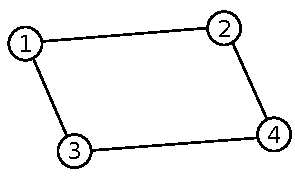
\includegraphics{network-example}
    \end{wrapfigure}

    Esimesena käivitatakse protseduur
    \begin{figure}[H]
        \centering
        \method{findRoute(4, 1, 4)}.
    \end{figure}

    Selle üks võimalik käitumine on
    \begin{figure}[H]
        \centering
        \method{ping(1, 4)}, mis tagastab $1$, \\
        \method{ping(1, 2)}, mis tagastab $0$, \\
        \method{ping(2, 4)}, mis tagastab $0$.
    \end{figure}

    Sellest infost piisab, et järeldada, et üks võimalik lühim tee arvutist
    $1$ arvutisse $4$ on $1 \to 2 \to 4$, mida kirjeldatakse järgmiselt:
    \begin{figure}[H]
        \centering
        \method{travelTo(2)}, \\
        \method{travelTo(4)}, \\
        \method{findRoute} lõpetab töö.
    \end{figure}

    \Scoring

    Kõigis alamülesannetes kehtib $2 \le N \le 1\,000$.

    \begin{description}
        \item[Alamülesanne 1 (25 punkti):] iga kahe arvuti vahel
            on täpselt üks lühim tee; $M$ ei või ületada $2N$.
        \item[Alamülesanne 2 (25 punkti):] $M$ ei või ületada $N^2$.
        \item[Alamülesanne 3 (25 punkti):] $M$ ei või ületada $4N$.
        \item[Alamülesanne 4 (25 punkti):] $M$ ei või ületada $2N$.
    \end{description}

    \Constraints

    \begin{description}
        \item[Ajalimiit:] 1 s.
        \item[Mälulimiit:] 64 MB.
    \end{description}

    \Experimentation

    Sinu arvutis olev hindamisprogramm loeb andmed standardsisendist.
    Sisendi esimesel real peavad olema neli täisarvu: $N$, $a$, $b$ ja
    \method{ping} käivituste arvu limiit $M$. Järgmisel $N$ real peab
    igaühel olema $N$ täisarvu, mis kirjeldavad arvutite vahelisi ühendusi:
    selle bloki $i$. rea $j$. positsioonil ($i \neq j$) olev arv näitab,
    mitut vahejaama arvutitst $i$ arvutisse $j$ saadetud sõnum läbib
    ($i$. rea $i$. positsioonil oleva arvu väärtus pole oluline).

    Sisend, mis vastab eelkirjeldatud näitele ja kehtestab $M$ limiidiks
    $100$:
    \begin{center}
        \begin{tabular}{p{4cm}}
            {\tt
                4 1 4 100 \newline
                0 0 0 1 \newline
                0 0 1 0 \newline
                0 1 0 0 \newline
                1 0 0 0
            }
        \end{tabular}
    \end{center}

\end{document}
